\documentclass[11pt,a4paper]{article}
\usepackage[utf8]{inputenc}
\usepackage[spanish]{babel}
\usepackage{graphicx}
\usepackage{hyperref}
\usepackage{amsmath}
\usepackage{booktabs}
\usepackage[margin=2.5cm]{geometry}
\usepackage{caption}
\usepackage{subcaption}

\title{\textbf{Explicabilidad y Detección de Shortcut Learning en Clasificación de Neumonía por Rayos X}}
\author{Proyecto Final - Ethics and Explainable AI}
\date{Diciembre 2025}

\begin{document}

\maketitle

\begin{abstract}
    Este trabajo investiga la aplicabilidad de técnicas de Inteligencia Artificial Explicable (XAI) en la detección de neumonía mediante imágenes de rayos X torácicos. Se entrena un modelo baseline basado en ResNet-18 preentrenado y se compara con un modelo intencionalmente afectado por \textit{shortcut learning}. Mediante técnicas como Grad-CAM y Activation Maximization, se demuestran diferencias en las características aprendidas por ambos, y cómo éstas no son evidentes mediante métricas tradicionales (como \textit{accuracy} en un cierto conjunto de datos). Los resultados subrayan la importancia crítica de XAI en aplicaciones médicas para garantizar que los modelos aprendan patrones clínicamente relevantes.
\end{abstract}

\section{Introducción}

La aplicación de deep learning en diagnóstico médico ha mostrado resultados prometedores, pero plantea desafíos éticos y de confiabilidad \cite{rudin2019stop}. Los modelos pueden aprender correlaciones espurias (\textit{shortcut learning}) \cite{geirhos2020shortcut} en lugar de patrones clínicamente relevantes, comprometiendo su generalización y seguridad.

Este proyecto tiene tres objetivos principales: (1) desarrollar un modelo de clasificación de neumonía interpretable, (2) demostrar experimentalmente el fenómeno de shortcut learning mediante corrupción controlada de datos, y (3) validar técnicas XAI para detectar estos comportamientos no deseados.

\section{Datos y Metodología}

\subsection{Dataset}

Se utiliza el dataset Chest X-Ray Pneumonia de Kaggle \cite{kermany2018chest}, que contiene 5.856 radiografías torácicas en escala de grises con dos clases: NORMAL (27\%) y PNEUMONIA (73\%). La distribución presenta un desbalance significativo de 2.71:1 a favor de la clase PNEUMONIA.

Los datos se dividen en 85\% entrenamiento (4,434 imágenes), 15\% validación (782 imágenes) y un conjunto de test fijo (624 imágenes). Las imágenes presentan dimensiones variables (384-2916 píxeles de ancho), requiriendo redimensionamiento a 224×224 píxeles para compatibilidad con ResNet-18.

\subsection{Arquitectura del Modelo}

Se emplea ResNet-18 preentrenado en ImageNet \cite{he2016deep}, modificando la capa final para clasificación binaria. El preentrenamiento proporciona características visuales robustas que facilitan el transfer learning. Durante el entrenamiento se aplica:

\begin{itemize}
    \item Data augmentation: flip horizontal (p=0.5), rotación (±10°), jitter de brillo/contraste
    \item Optimizador: AdamW con learning rate inicial de $10^{-4}$ y decaimiento de peso (\textit{weight decay}) de $10^{-4}$
    \item Función de pérdida: CrossEntropyLoss con pesos de clase balanceados
    \item Early stopping con paciencia de 10 épocas
\end{itemize}

\subsection{Generación de Shortcut Learning}

Para estudiar el fenómeno de forma controlada, se crea un segundo modelo entrenado desde cero (sin preentrenamiento \footnote{En pruebas iniciales, se intentó hacer con preentrenamiento, pero el modelo no aprendía los atajos deseados (probablemenente debido a que ya había aprendido características robustas que impedían la dependencia de atajos espurios durante el preentrenamiento)}) sobre un dataset corrupto. Se añaden marcadores circulares blancos en la esquina superior izquierda únicamente a imágenes de la clase PNEUMONIA durante entrenamiento. Este artefacto artificial actúa como un \textit{shortcut} espurio correlacionado perfectamente con la clase objetivo.

\begin{figure}[h]
    \centering
    \includegraphics[width=0.65\textwidth]{figures/04_corruption_comparison.png}
    \caption{Ejemplos de imágenes originales vs. corruptas con marcador artificial}
    \label{fig:corruption}
\end{figure}

\subsection{Entrenamiento y Evaluación}

Ambos modelos (baseline y shortcut) se entrenan, respectivamente, durante 20 y 15 épocas hasta convergencia. De cara a diagnosticar un posible sobreajuste, se monitorean las curvas de pérdida y accuracy en entrenamiento y validación (Figura \ref{fig:overfitting_sub1}). Adicionalmente, se evalúa el rendimiento en datos limpios y corruptos para cuantificar el impacto del shortcut learning. Como podemos observar en la Figura \ref{fig:overfitting_sub2}, el modelo baseline alcanza un accuracy del 81.57\% en datos limpios, mientras que el modelo shortcut logra un 98.88\% en datos corruptos pero sólo un 46.47\% en datos limpios, evidenciando su dependencia del marcador artificial.

\begin{figure}[h!]
    \centering

    % Fila superior: dos imágenes lado a lado
    \begin{subfigure}[c]{0.48\textwidth}
        \centering
        \includegraphics[width=\textwidth]{figures/06_overfitting_check.png}
        \caption{Evolución de las funciones de pérdida y accuracy durante el entrenamiento (Baseline)}
        \label{fig:overfitting_sub1}
    \end{subfigure}
    \hfill
    \begin{subfigure}[c]{0.48\textwidth}
        \centering
        \includegraphics[width=\textwidth]{figures/07_shortcut_learning_comparison.png}
        \caption{Comparación de rendimiento entre modelo baseline y shortcut}
        \label{fig:overfitting_sub2}
    \end{subfigure}
    \caption{Análisis de sobreajuste y rendimiento entre modelos}
    \label{fig:overfitting}
\end{figure}

\section{Técnicas XAI Aplicadas}

De cara a interpretar y comparar ambos modelos, hemos seleccionado dos técnicas de XAI, una local/híbrida (Grad-CAM) y otra global (Activation Maximization):

\subsection{Grad-CAM (Gradient-weighted Class Activation Mapping)}

Grad-CAM visualiza las regiones de una imagen concreta que más contribuyen a la decisión del modelo mediante el cálculo de gradientes de la clase objetivo respecto a los mapas de activación de la última capa convolucional. Los resultados muestran diferencias claras entre ambos modelos (Figura \ref{fig:gradcam}).

% \begin{figure}[h]
%     \centering
%     \includegraphics[width=0.9\textwidth]{reports/figures/08_gradcam_pneumonia_case1.png}
%     \caption{Comparación Grad-CAM entre modelo baseline y shortcut en casos de neumonía}
%     \label{fig:gradcam}
% \end{figure}

El modelo baseline enfoca correctamente en regiones pulmonares centrales, mientras que el modelo corrupto concentra su atención exclusivamente en la esquina superior izquierda donde se ubica el marcador artificial.

% \begin{figure}[h]
%     \centering
%     \includegraphics[width=0.9\textwidth]{reports/figures/08_gradcam_pneumonia_case1.png}
%     \caption{Comparación Grad-CAM entre modelo baseline y shortcut en casos de neumonía}
%     \label{fig:gradcam}
% \end{figure}

\subsection{Activation Maximization}

Esta técnica genera imágenes sintéticas que maximizan la activación de cada clase mediante ascenso de gradiente. Para el modelo baseline, los prototipos de la clase NORMAL muestran patrones de costillas y estructuras anatómicas reconocibles, mientras que los prototipos de PNEUMONIA presentan texturas complejas de bajo nivel menos interpretables.

En contraste, el modelo shortcut genera prototipos sin estructuras anatómicas claras. Los scores de confianza son significativamente menores (2.5 para NORMAL, -2.6 para PNEUMONIA) comparados con el baseline (13 para NORMAL, 40 para PNEUMONIA). El score negativo para PNEUMONIA indica la incapacidad del modelo para generar ejemplos de esta clase sin el marcador artificial.

\subsection{Análisis de Atención en Múltiples Ejemplos}

El análisis sistemático de Grad-CAM sobre múltiples muestras revela patrones consistentes:

\begin{itemize}
    \item \textbf{Modelo Baseline}: Atención distribuida en áreas pulmonares bilaterales, identificando opacidades y consolidaciones coherentes con presentación clínica de neumonía
    \item \textbf{Modelo Shortcut}: Atención invariablemente concentrada en la región del marcador artificial, independientemente del contenido médico de la imagen
\end{itemize}

\section{Sanity Checks y Actionable Insights}

\subsection{Validación mediante Sanity Checks}

Se implementan dos sanity checks fundamentales para validar la fidelidad de las explicaciones XAI:

\textbf{1. Randomization Test:} Se reemplazan progresivamente los pesos del modelo por valores aleatorios, comenzando desde las capas superiores. Las explicaciones del modelo baseline pierden coherencia gradualmente conforme aumenta la aleatorización, confirmando que Grad-CAM refleja genuinamente el proceso de decisión aprendido.

\textbf{2. Baseline Comparison:} Se comparan las explicaciones con un modelo con pesos completamente aleatorios. El modelo entrenado muestra mapas de atención estructurados y consistentes, mientras que el modelo aleatorio produce mapas de ruido sin patrones discernibles.

\subsection{Métricas de Rendimiento}

El contraste entre ambos modelos es evidente en el desempeño sobre datos limpios vs. corruptos:

\begin{table}[h]
    \centering
    \begin{tabular}{lcc}
        \toprule
        \textbf{Modelo} & \textbf{Acc. Datos Limpios} & \textbf{Acc. Datos Corruptos} \\
        \midrule
        Baseline        & 87.5\%                      & -                             \\
        Shortcut        & 46.5\%                      & 98.9\%                        \\
        \bottomrule
    \end{tabular}
    \caption{Comparación de rendimiento entre modelos}
\end{table}

La precisión del modelo shortcut en datos limpios (46.5\%) es inferior incluso a un clasificador aleatorio (50\%), confirmando que el modelo no aprendió características relevantes de neumonía sino únicamente la correlación con el marcador artificial.

\subsection{Actionable Insights para Aplicaciones Médicas}

Este estudio genera recomendaciones prácticas:

\begin{enumerate}
    \item \textbf{Validación obligatoria con XAI}: Todo modelo médico debe evaluarse con técnicas de explicabilidad antes del despliegue clínico
    \item \textbf{Inspección de datos}: Los datasets médicos deben auditarse para detectar correlaciones espurias (marcadores institucionales, artefactos de adquisición, sesgos demográficos)
    \item \textbf{Transfer learning con precaución}: El preentrenamiento en ImageNet aporta robustez contra shortcuts, pero no elimina completamente el riesgo
    \item \textbf{Evaluación en distribuciones múltiples}: Los modelos deben validarse en datos de diferentes instituciones y equipos radiológicos
\end{enumerate}

\section{Limitaciones y Discusión}

\subsection{Limitaciones del Estudio}

\textbf{Interpretabilidad humana vs. fidelidad}: Las visualizaciones Grad-CAM son plausibles para humanos pero pueden no capturar completamente el razonamiento del modelo. La diferencia entre \textit{faithfulness} y \textit{plausibility} es una limitación inherente a técnicas de explicabilidad en visión por computadora.

\textbf{Simplificación experimental}: El shortcut introducido (marcador circular) es deliberadamente obvio. Los shortcuts reales en datasets médicos suelen ser más sutiles (diferencias en contraste institucional, textos en imágenes, patrones de compresión).

\textbf{Tamaño del dataset}: Con 5,856 imágenes, el dataset es relativamente pequeño para estándares de deep learning. Estudios clínicos requerirían validación en decenas de miles de casos.

\subsection{Implicaciones Éticas}

El fenómeno de shortcut learning en IA médica plantea serias preocupaciones éticas. Un modelo que clasifica basándose en artefactos en lugar de patología real podría:

\begin{itemize}
    \item Fallar catastróficamente al ser desplegado en instituciones con diferentes equipos/protocolos
    \item Generar falsa confianza en profesionales médicos al mostrar alta precisión en validación
    \item Perpetuar sesgos si los shortcuts correlacionan con demografías específicas
\end{itemize}

La obligatoriedad de XAI en sistemas médicos de alto riesgo no es solo una mejor práctica técnica, sino un imperativo ético para garantizar seguridad del paciente.

\section{Conclusiones}

Este proyecto demuestra experimentalmente la efectividad de técnicas XAI para detectar shortcut learning en clasificación de imágenes médicas. Los resultados principales son:

\begin{enumerate}
    \item El modelo baseline basado en transfer learning aprende características anatómicas relevantes, evidenciado por Grad-CAM que enfoca en regiones pulmonares y Activation Maximization que genera prototipos con estructuras reconocibles

    \item El modelo shortcut, entrenado desde cero con datos corruptos, depende exclusivamente del marcador artificial, alcanzando 98.9\% de precisión en datos corruptos pero solo 46.5\% en datos limpios

    \item Los sanity checks validan que las explicaciones XAI reflejan fielmente el razonamiento aprendido por los modelos

    \item El preentrenamiento en ImageNet proporciona robustez contra shortcuts simples, aunque no es una solución universal
\end{enumerate}

En conclusión, XAI no es opcional en aplicaciones médicas de IA: es una necesidad técnica y ética para garantizar que los modelos aprendan patrones clínicamente relevantes en lugar de correlaciones espurias. La combinación de múltiples técnicas de explicabilidad (Grad-CAM, Activation Maximization, sanity checks) proporciona una visión más completa y confiable del comportamiento del modelo.

\appendix

\section{Ilustraciones Adicionales}

Si bien no incluimos todas las figuras en el cuerpo principal del informe (en pos de la brevedad), proponemos una serie de ilustraciones complementarias que pueden facilitar la comprensión de los conceptos tratados:

\begin{figure}[htbp]
    \centering

    % Fila superior: dos imágenes lado a lado
    \begin{subfigure}[b]{0.48\textwidth}
        \centering
        \includegraphics[width=\textwidth]{figures/01_class_distribution.png}
        \caption{Distribución de clases en el dataset}
        \label{fig:sub1}
    \end{subfigure}
    \hfill
    \begin{subfigure}[b]{0.48\textwidth}
        \centering
        \includegraphics[width=\textwidth]{figures/02_image_properties.png}
        \caption{Propiedades de las imágenes (tamaños y formatos)}
        \label{fig:sub2}
    \end{subfigure}

    % Salto de línea
    \vspace{0.5cm}

    % Fila inferior: una imagen más ancha
    \begin{subfigure}[b]{0.9\textwidth}
        \centering
        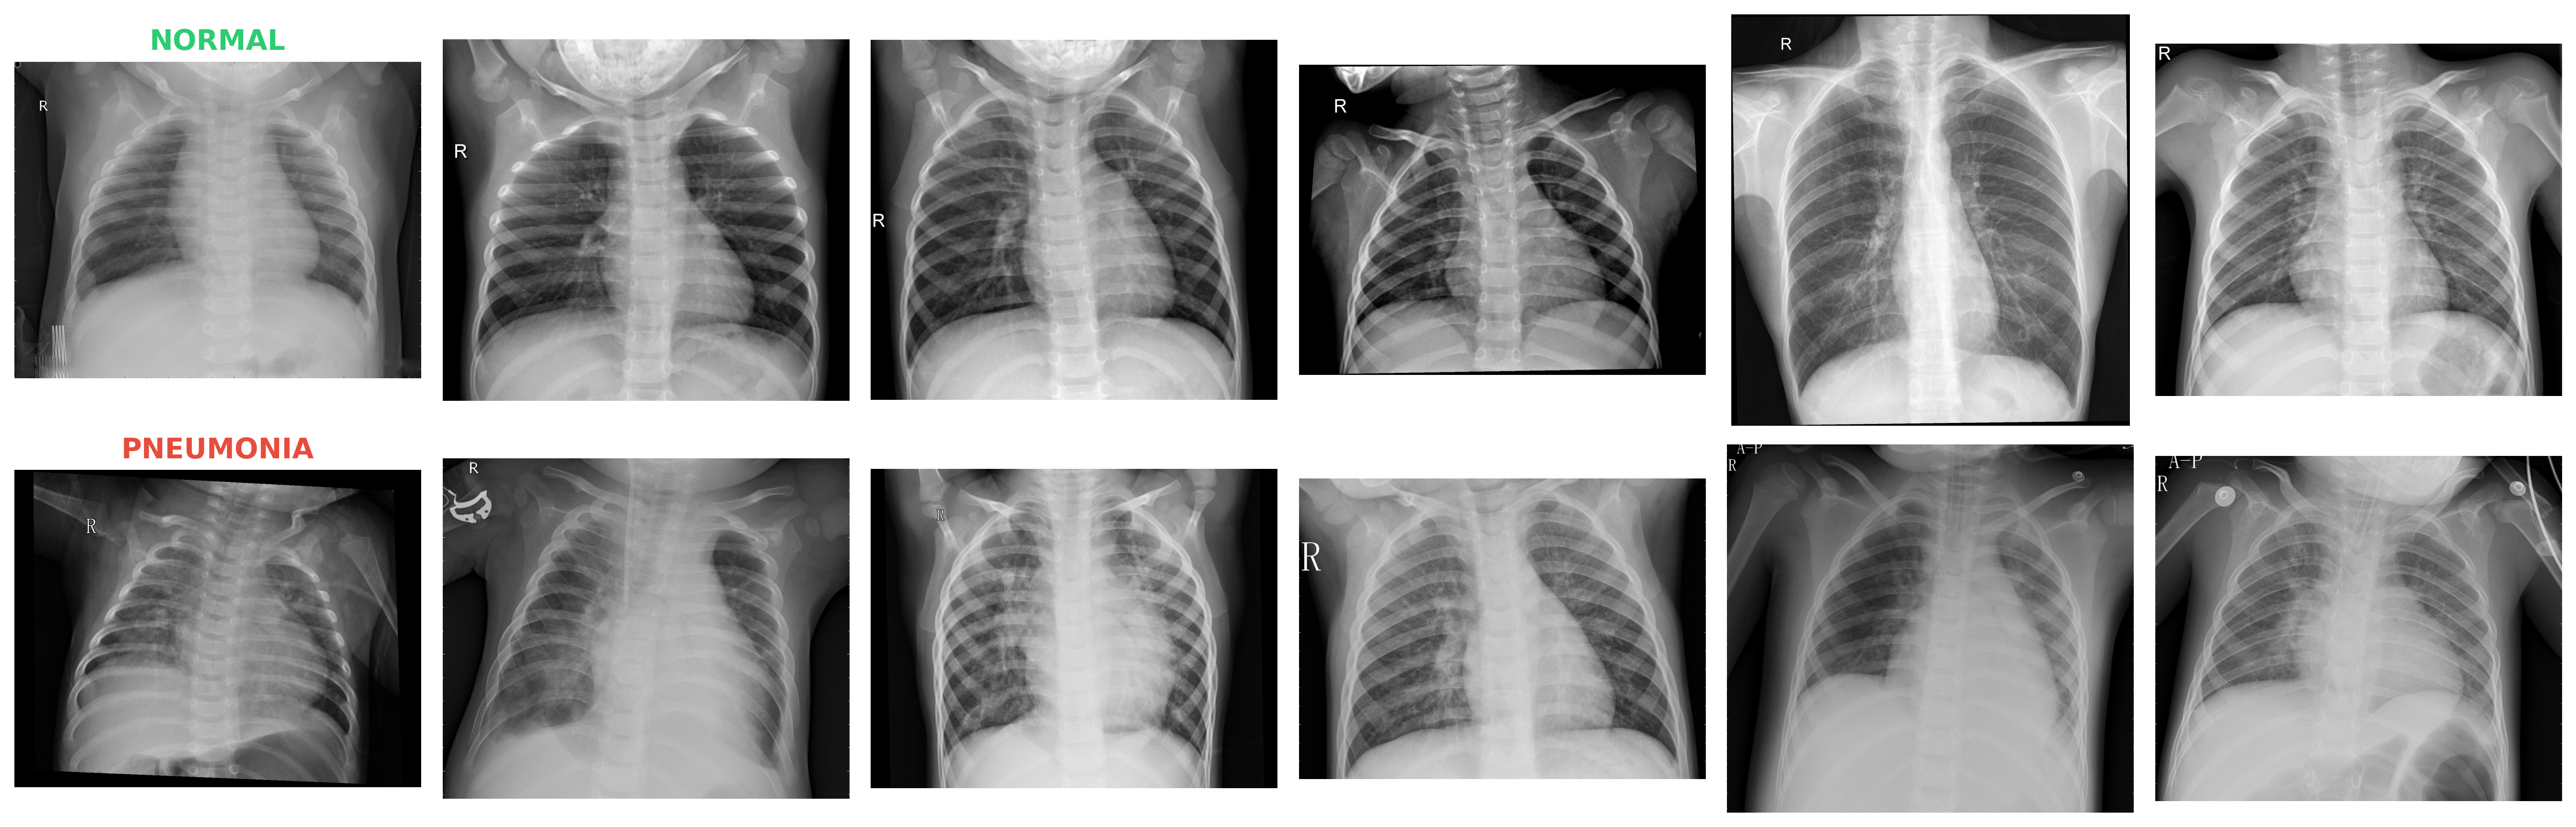
\includegraphics[width=\textwidth]{figures/03_sample_images.png}
        \caption{Imágenes de muestra del dataset}
        \label{fig:sub3}
    \end{subfigure}

    \caption{Información visual adicional sobre el dataset utilizado}
    \label{fig:tres_imagenes}
\end{figure}

\bibliographystyle{plain}
\bibliography{citations}

\end{document}
